Simulation is defined in \cite{banks2010} as \begin{quote} \emph{the imitation of the operation of a real-world process or system over time.} \end{quote}
There are many types of simulation, varying in the methods used and the type of systems being analyzed.
For instance, a simulation can be \emph{deterministic}, or \emph{stochastic}, depending on whether random variables are involved or not.
The first step in a simulation is usually to formulate the problem and the corresponding model -- here, assumptions will be made about the system being studied. 
This might include deciding which variables to ignore, or assuming how an input is distributed probabilistically.

In the previous sections, we discussed how to generate random variables in Excel, using a few of the most common probability distributions.
Before working on examples of simulations, we first discuss \textbf{data tables} in Excel.

\section{Data Tables in Excel}\label{sec3:datatable}

In Excel, data tables are used for scenario analysis.
They show the output of a calculation for different values of an input (similar to performing a sensitivity analysis).
We demonstrate this using an example.

\begin{myexample}\label{ex:3_datatable}
Suppose that you open a savings account at your bank on January 1 of this year, that earns you a fixed rate of 3\% per year.
If you deposit \$1,000 on January 1, at the end of the year you will have \$1,030.
What happens if we change the initial amount deposited?

Consider the following Excel spreadsheet: in cell \texttt{B2} we enter the initial amount deposited; \texttt{B3} has the interest earned (with formula \texttt{= 0.03 * B2}); \texttt{B4} has the total amount \texttt{= B2 + B3}.

To begin constructing the data table, in cells \texttt{D3:D14} input the different deposit amounts you would like to check (from \$900 to \$2,000).
In cell \texttt{E2} enter the formula \texttt{=B4}.

\begin{figure}[htbp]
	\centering
	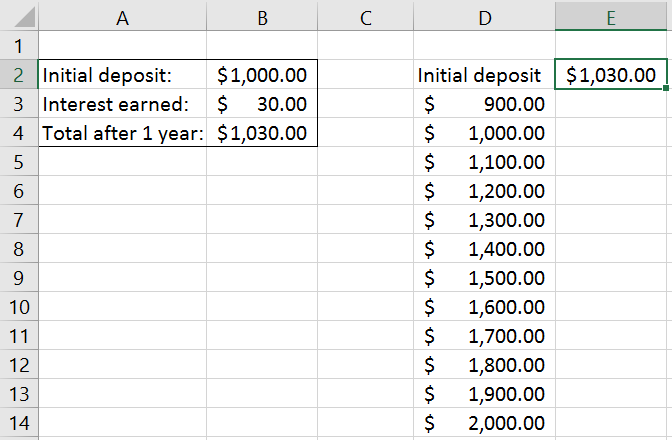
\includegraphics[width=0.45\textwidth]{fig/3_datatable_1.png}
	\label{fig:3_datatable_1}
\end{figure}

Now highlight cells \texttt{D2:E14}, and click `Data Table' (Data $\rightarrow$ What-If Analysis $\rightarrow$ Data Tables).
For `Column input cell' enter the cell corresponding to the initial deposit, \texttt{B2}, then click OK.

\begin{figure}[htbp]
	\centering
	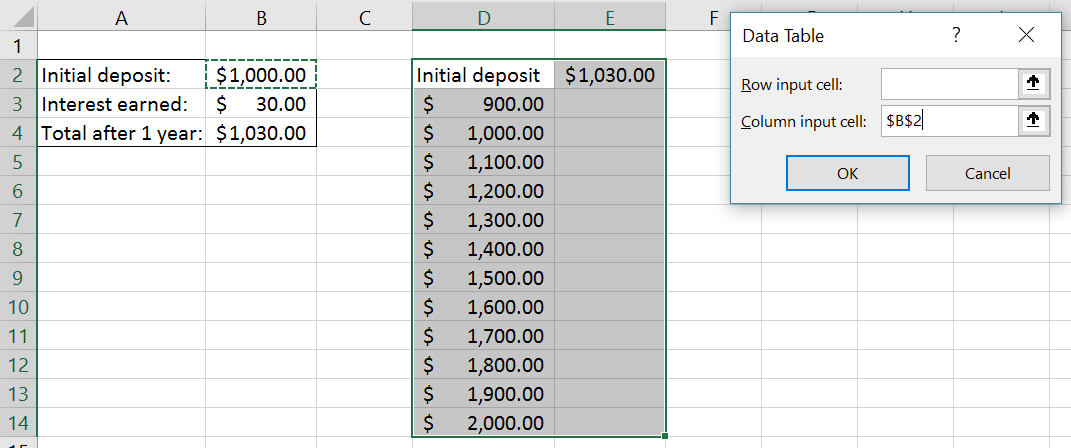
\includegraphics[width=0.75\textwidth]{fig/3_datatable_2.png}
	\label{fig:3_datatable_2}
\end{figure}

The cells beside the input column will be populated with the one-year totals for each corresponding initial deposit.

\begin{figure}[htbp]
	\centering
	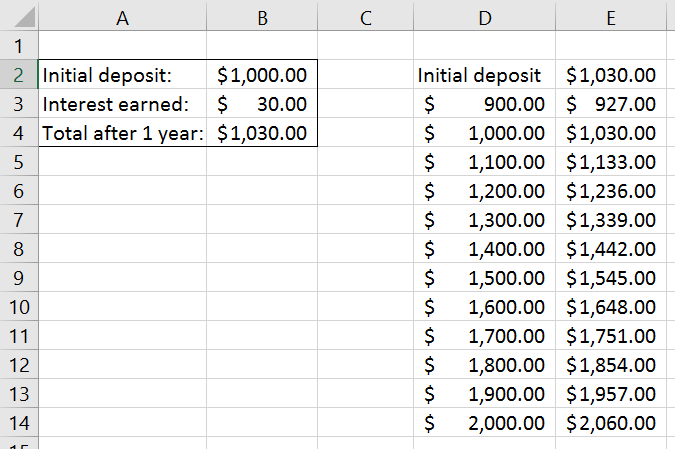
\includegraphics[width=0.5\textwidth]{fig/3_datatable_3.png}
	\label{fig:3_datatable_3}
\end{figure}

\end{myexample}

Data tables do the work of entering information and recalculating the worksheet based on the changes.
Example~\ref{ex:3_datatable} demonstrated a \emph{one-way data table}, because one input variable was allowed to vary.
We can also construct \emph{two-way data tables}.

\begin{myexample}\label{ex:3_datatable2}
Continuing the previous example, suppose that you wanted to compute your year-end savings account balance given different interest rates for the account.
To do this using a two-way data table, see the following spreadsheet:

\begin{figure}[htbp]
	\centering
	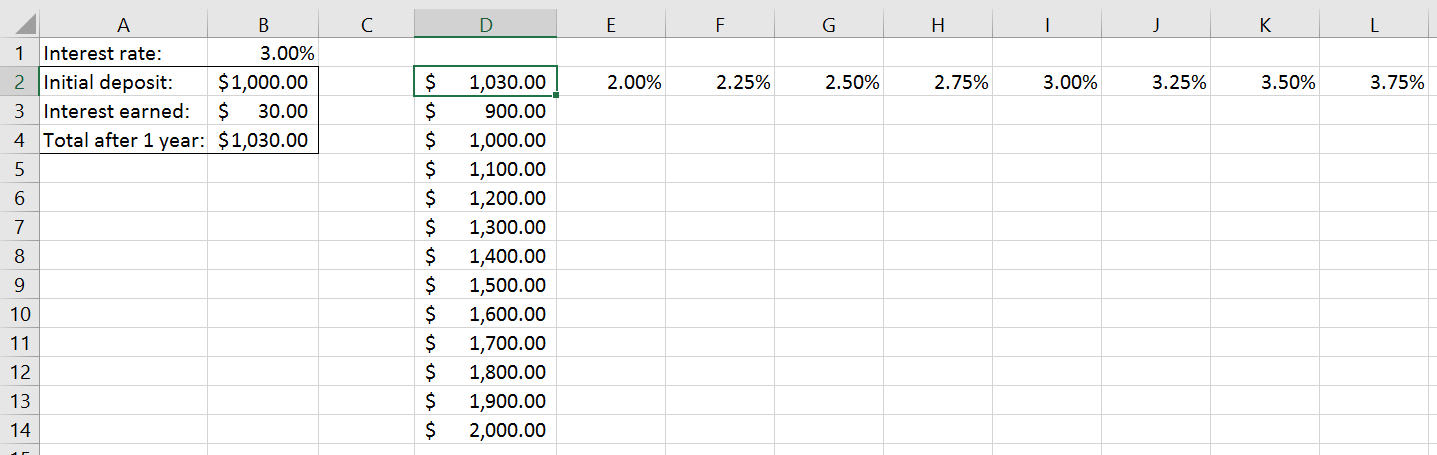
\includegraphics[width=0.9\textwidth]{fig/3_datatable2_1.png}
	\label{fig:3_datatable2_1}
\end{figure}

Enter the formula \texttt{=B4} in cell \texttt{D2}, and also change cell \texttt{B3} to the formula \texttt{=B1*B2}, to account for a varying interest rate.
In cells \texttt{E2:L2} enter the different interest rates under consideration.
Now highlight cells \texttt{D2:L14}, and click Data Table.
For `Column input cell' enter \texttt{B2}, and for `Row input cell' enter \texttt{B1}.

\begin{figure}[htbp]
	\centering
	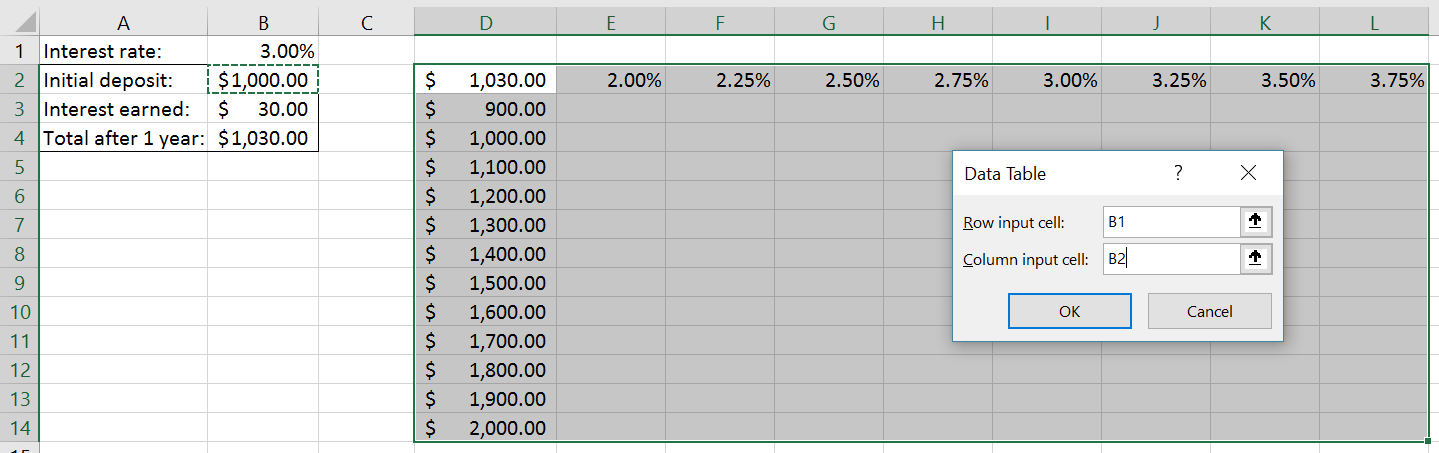
\includegraphics[width=0.9\textwidth]{fig/3_datatable2_2.png}
	\label{fig:3_datatable2_2}
\end{figure}

Click OK.
The table should now be populated with the different year-end totals for the given combinations of initial deposit and interest rate.

\begin{figure}[htbp]
	\centering
	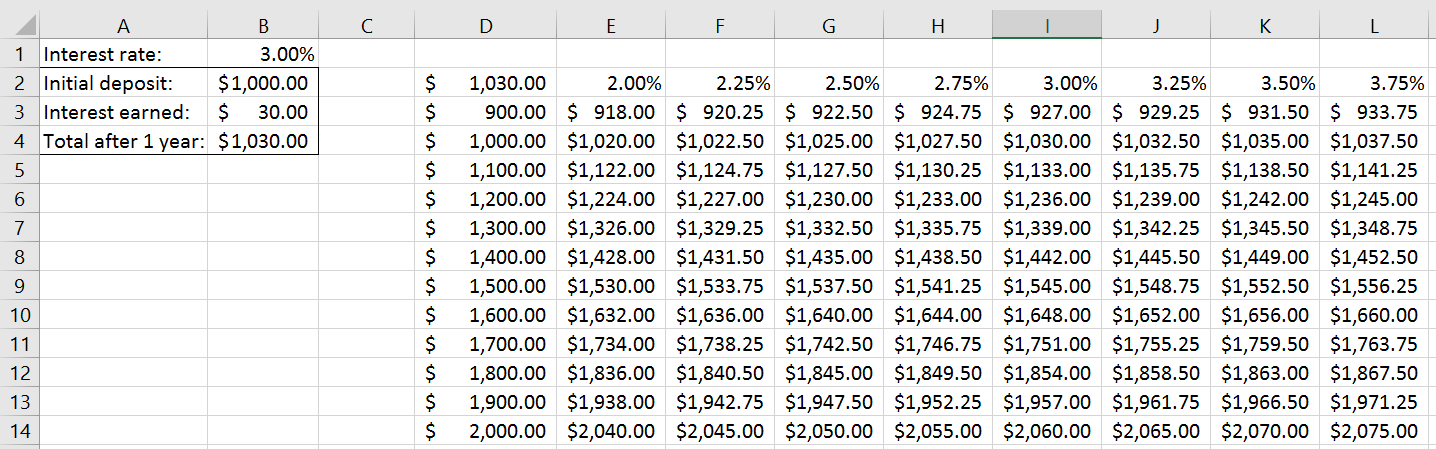
\includegraphics[width=0.9\textwidth]{fig/3_datatable2_3.png}
	\label{fig:3_datatable2_3}
\end{figure}


\end{myexample}

Rather than looking at an evenly-spaced set of input values, we can also construct tables based on random inputs to help us develop intuition for what the transformed random output should look like.

Note that Examples~\ref{ex:3_datatable} and ~\ref{ex:3_datatable2} are \emph{deterministic}: each entry has a value that is 
computed directly from its inputs, and repeating the calculation will produce an identical result.
The following example, on the other hand, is \emph{stochastic}: it incorporates some randomness.


\begin{myexample}\label{ex:3_datatable3}
Suppose that your initial deposit amount is a normally-distributed random variable with mean \$1,000 and standard deviation \$100.
In cell \texttt{B2}, following the discussion in Section~\ref{sec2:normal} we enter the formula \texttt{=NORM.INV(RAND(),1000,100)}.
To initialize the data table cell \texttt{E2} still refers to \texttt{B4}, while the first column can just have trial numbers (say we want to run this experiment 10 times).

\begin{figure}[htbp]
	\centering
	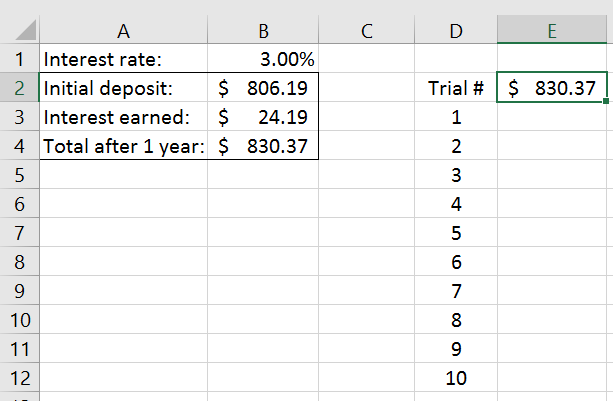
\includegraphics[width=0.4\textwidth]{fig/3_datatable3_1.png}
	\label{fig:3_datatable3_1}
\end{figure}

Highlight cells \texttt{D2:E12}, then click Data Table.
Now for `Column input cell' choose any blank cell.
The value in \texttt{B2}, and hence the output \texttt{B4}, will change each time the worksheet is recalculated so we do not need to specify a changing input cell.

\begin{figure}[htbp]
	\centering
	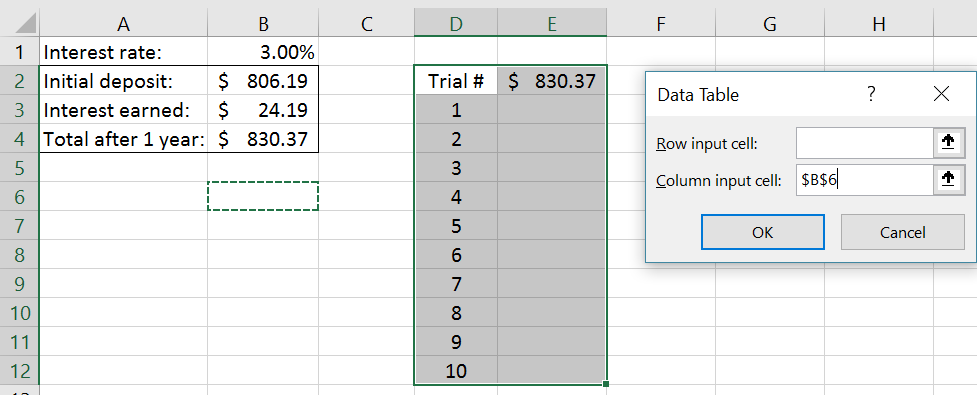
\includegraphics[width=0.7\textwidth]{fig/3_datatable3_2.png}
	\label{fig:3_datatable3_2}
\end{figure}

Click OK.
Now the table is populated by the different year-end values obtained given the assumption on the initial deposit.

\begin{figure}[htbp]
	\centering
	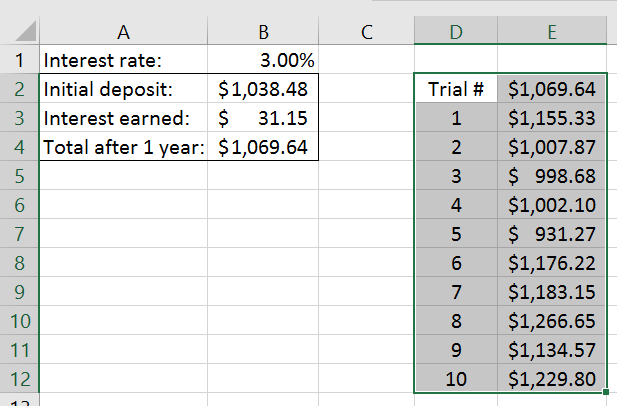
\includegraphics[width=0.5\textwidth]{fig/3_datatable3_3.png}
	\label{fig:3_datatable3_3}
\end{figure}
 

\end{myexample}

Now we begin our foray into simulation by looking at some simple problems.


\section{A Beginning Example -- Coin-Flipping}\label{sec3:begin}

The following problem recently appeared on the blog \emph{The Riddler}\footnote{A weekly puzzle blog on the site \texttt{http://www.fivethirtyeight.com}.}:

\begin{quote}
You and I find ourselves indoors one rainy afternoon, with nothing but some loose change in the couch cushions to entertain us. We decide that we'll take turns flipping a coin, and that the winner will be whoever flips 10 heads first. The winner gets to keep all the change in the couch! Predictably, an enormous argument erupts: We both want to be the one to go first.

What is the first flipper's advantage? In other words, what percentage of the time does the first flipper win this game?\footnote{\url{https://fivethirtyeight.com/features/can-you-time-the-stoplight-just-right/}, \\ January 20, 2017}
\end{quote}

This is a question about probability, and if you have taken some courses in probability and statistics, then you will  have seen exercises like this.
The exact probability that the first flipper wins the game can be computed analytically, but this is not easy to do.
However, the process is very simple to simulate.

To simulate the coin flips, we use a Bernoulli random variable with a $p = 0.50$ probability of heads.
Using 100 flips each, we keep track of the number of heads for each player, and compare the number of flips needed to get to 10.
Note that we have to cap the number of flips at a certain point, even though in theory there is a nonzero probability that neither player gets at least 10 heads in the first 100 flips.\footnote{Compute this probability using the inverse binomial function in Excel!}

\begin{figure}[htbp]
	\centering
	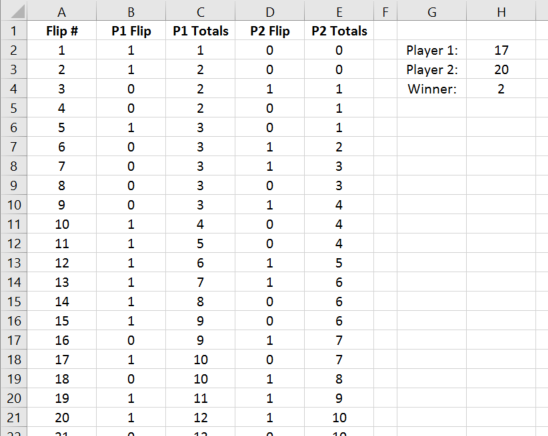
\includegraphics[width=0.7\textwidth]{fig/3_couch_1.png}
	\label{fig:3_couch_1}
\end{figure}

The formulas we use are: \texttt{RANDBETWEEN(0,1)} to generate the coin flips, and \texttt{SUM(\$B\$2:B2)} and \texttt{SUM(\$D\$2:D2)} for the running totals (autofilled).

To output the number of flips to get to 10, we use the \texttt{MATCH(lookup\_value, lookup\_array, [match\_type])} function in Excel, which finds the first occurrence of \texttt{lookup\_value} in the array \texttt{lookup\_array}, with parameter \texttt{match\_type} equal to 1, 0, or -1 depending on whether you want \texttt{MATCH} to find the first value less than or equal to, equal to, or greater than or equal to the lookup value, respectively.

In the spreadsheet shown, cell \texttt{H2} has the formula \texttt{MATCH(10,C2:C101,0)}, and cell \texttt{H3} has formula \texttt{MATCH(10,E2:E101,0)}.
In this run Player 1 gets 10 heads on the 17th flip, while Player 2 gets 10 heads on the 20th.
Lastly, in \texttt{H4} we enter the formula \texttt{IF(H2<=H3,1,2)}.


\begin{figure}[htbp]
	\centering
	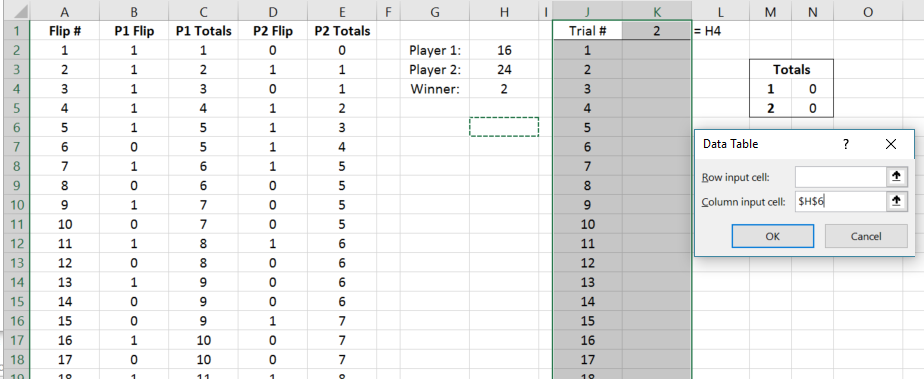
\includegraphics[width=0.9\textwidth]{fig/3_couch_2.png}
	\label{fig:3_couch_2}
\end{figure}

To run this multiple times, we use a data table with 500 rows. 
We set a blank cell as the column input cell, as explained in Example~\ref{ex:3_datatable3}.

\begin{figure}[htbp]
	\centering
	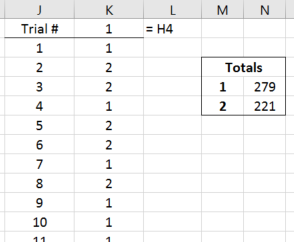
\includegraphics[width=0.4\textwidth]{fig/3_couch_3.png}
	\label{fig:3_couch_3}
\end{figure}

Our results give 279 wins for Player 1, and 221 wins for Player 2.
Hence our simulation approximates the probability of Player 1 winning as $53.8\%$.
The actual probability is given by the expression \[ \sum_{n = 10}^\infty \left[\frac{1}{2^n}\frac{(n-1)!}{9!(n-10)!}  \left( 1 - \sum_{i=10}^{n-1} \frac{1}{2^i}\frac{(i-1)!}{9!(i-10)!}\right) \right] \approx 53.2909\%. \]
This is in some sense a ``lucky'' result, if you repeat the calculation you will see that it is usually not so accurate.

\section{Generating Permutations and Sampling without Replacement}

Here is another puzzle from \emph{The Riddler}:

\begin{quote}
On snowy afternoons, you like to play a solitaire `game' with a standard, randomly shuffled deck of 52 cards.
You start dealing cards face up, one at a time, into a pile.
As you deal each card, you also speak aloud, in order, the 13 card faces in a standard deck: ace, two, three, etc.
(When you get to king, you start over at ace.)
You keep doing this until the rank of the card you deal matches the rank you speak aloud, in which case you lose.
You win if you reach the end of the deck without any matches.

What is the probability you win?\footnote{\url{https://fivethirtyeight.com/features/can-you-deal-with-these-card-game-puzzles/}, \\ December 30, 2016.}
\end{quote}

One can compute solution exactly using combinatorics, but the calculation is difficult and subtle enough that the authors of the blog presented an oversimplified incorrect solution the following week, despite the fact that several people presumably sent the correct answer (while many others sent incorrect ones).\footnote{Original solution: \url{https://fivethirtyeight.com/features/dont-throw-out-that-calendar/}. \\ Correction: {\tiny \url{https://fivethirtyeight.com/features/how-long-will-it-take-to-blow-out-the-birthday-candles/\#correction}}. \\ Solution method: {\tiny \url{http://math.stackexchange.com/questions/1891958/derangements-of-a-deck-of-cards-where-ranks-are-equal}}, giving a probability of $1.6233\%$.}
Simulation can be a good sanity check on an analytic solution.
In this case, we would have to compute the solution quite accurately to spot the error.

To simulate this game, we need a way to generate a random arrangement of a 52-card deck.
Let us assign cards to numbers using the following scheme:

{ \small
\begin{center}	
\begin{tabular}{c|ccccccc}
& A & 2 & 3 & $\cdots$ & J & Q & K \\
\hline
$\spadesuit$ & 1 & 2 & 3 & $\cdots$ & 11 & 12 & 13 \\
$\vardiamond$ & 14 & 15 & 16 & $\cdots$ & 24 & 25 & 26 \\
$\varheart$ & 27 & 28 & 29 & $\cdots$ & 37 & 38 & 39 \\
$\clubsuit$ & 40 & 41 & 42 & $\cdots$ & 50 & 51 & 52 \\
\hline
(mod 13) & 1 & 2 & 3 & $\cdots$ & 11 & 12 & 0 
\end{tabular}
\end{center}
}

Note that we only have to consider these numbers modulo 13, since the suit is ignored.
Now we need to generate a random permutation of the numbers 1 to 52, corresponding to the shuffled deck of cards.

Refer to the spreadsheet below: first enter in cells \texttt{C2:C53} the numbers 1 to 52 -- this will correspond to the cards being announced.
Then, in the first column generate 52 random numbers using \texttt{RAND()}.
We then generate a permutation based on the relative positions of each cell in the array \texttt{A2:A53}.
To do this we enter in cell \texttt{B2} the formula \[\texttt{=INDEX(\$C\$2:\$C\$53,MATCH(LARGE(\$A\$2:\$A\$53,ROW()-ROW(\$A\$2)+1),\$A\$2:\$A\$53,0))}.\]
This instructs Excel to look for the $k$th largest entry in the array of random numbers, then output its relative position in that array.
Auto-filling the rest of the cells in \texttt{B2:B53} yields the random permutation.
In Figure~\ref{fig:3_deck_1}, for example, the first few cells in column B mean that the largest entry in column A is in the 6th position (\texttt{A7}), the second largest entry is in the 1st position (\texttt{A2}), and the third largest entry is in the 35th position.

\begin{figure}[htbp]
	\centering
	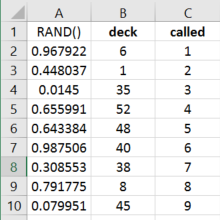
\includegraphics[width=0.25\textwidth]{fig/3_deck_1.png}
	\caption{Generating a random permutation in Excel. \label{fig:3_deck_1}}
\end{figure}

Observe that this method simulates sampling from a finite set without replacement, although generating a permutation is not practical for large sets.
Drawing only $k$ cards out of the deck without replacement corresponds to choosing the first $k$ entries in the permutation.

To check whether the drawn card matches the rank being called out, we just do a modulo check: \[ \texttt{=IF(MOD(B2,13)=MOD(C2,13),1,0)} \] will output 1 if the two ranks match, and 0 otherwise.
Summing up column C will result in the total number of times that the ranks match, so you win if this sum is zero.
Using a data table, we repeat this experiment 1000 times.


\begin{figure}[htbp]
	\centering
	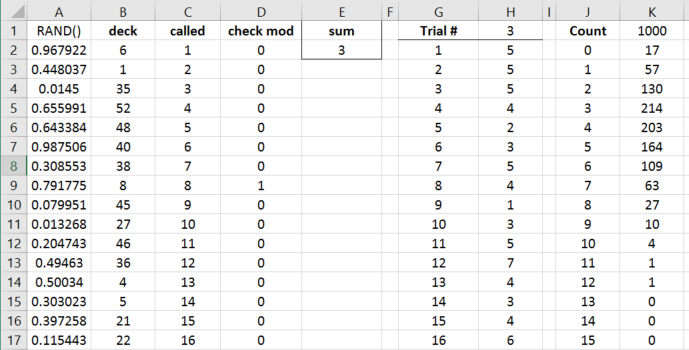
\includegraphics[width=0.8\textwidth]{fig/3_deck_2.png}
	\label{fig:3_deck_2}
\end{figure}

The \texttt{COUNTIF} function in Excel counts how many instances of 0, 1, and so on, appear in the data table; as the spreadsheet shows we won 17 times out of 1000 trials (so we estimate the probability to be $1.7\%$).
More trials will lead to greater accuracy in estimating the true probability, which as noted is around $1.62\%$.

\section{Random Walks}

A \textbf{random walk} is a path where each step depends on a probability distribution.
Random walks have many applications, from physics (Brownian motion) to finance (movement of stocks on the market).

\subsection{Random Walks on a Line} 
A \emph{1-dimensional random walk} is a path on the real number line that starts at $0$, and with probability $p$ moves one unit to the right, and with probability $1-p$ moves one unit to the left.
Here we consider the simplest case, where $p = 0.5$.
We can think of each step as being determined by a fair coin flip.

\begin{figure}[htbp]
	\centering
	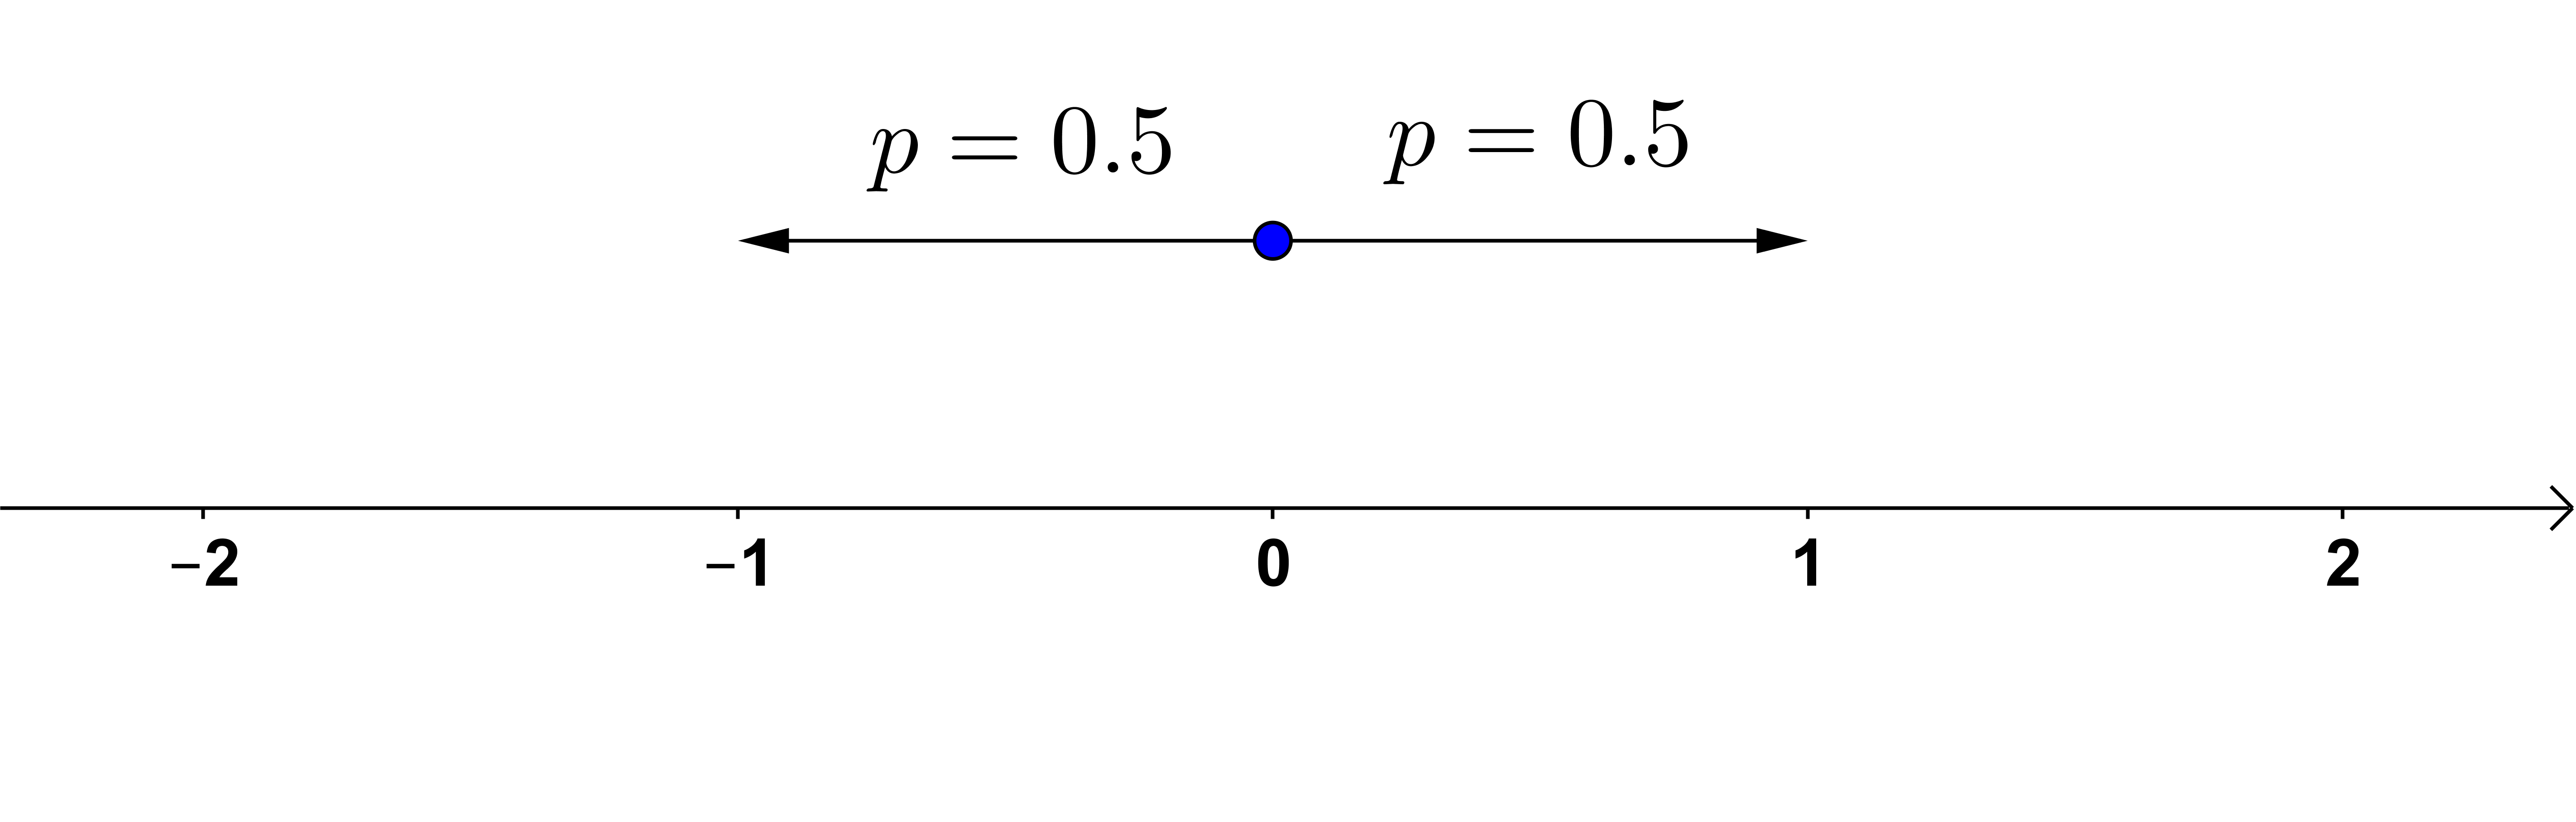
\includegraphics[width=0.5\textwidth]{fig/3_randomwalk_1.png}
	\label{fig:3_randomwalk_1}
\end{figure}

\vspace{-0.3cm}

This is easy to simulate in Excel, as shown in Figure~\ref{fig:3_randomwalk_2}.
Verify for yourself that the formula shown outputs \texttt{B1}$-1$ or \texttt{B1}$+1$ with equal probability.
Using the Chart function produces a visual of the random walk produced.

\begin{figure}[htbp]
	\centering
	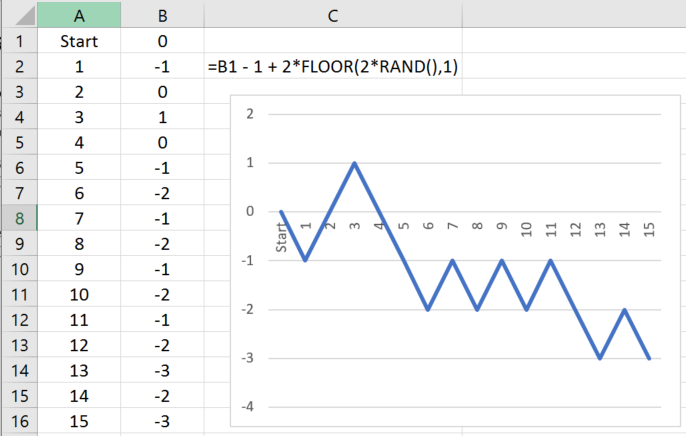
\includegraphics[width=0.6\textwidth]{fig/3_randomwalk_2.png}
	\caption{Generating a random walk in Excel \label{fig:3_randomwalk_2}}
\end{figure}

A basic problem about random walks is whether they return to their starting point.
Let us generate random walks (using data tables) and then count what fraction of those generated do return to 0.
The next two figures show the results of generating a thousand random walks of length 100 and 1000, respectively.
Note the usage of the \texttt{MATCH} function to look for the first occurrence of zero in the walk.

\begin{figure}[htbp!]
	\centering
	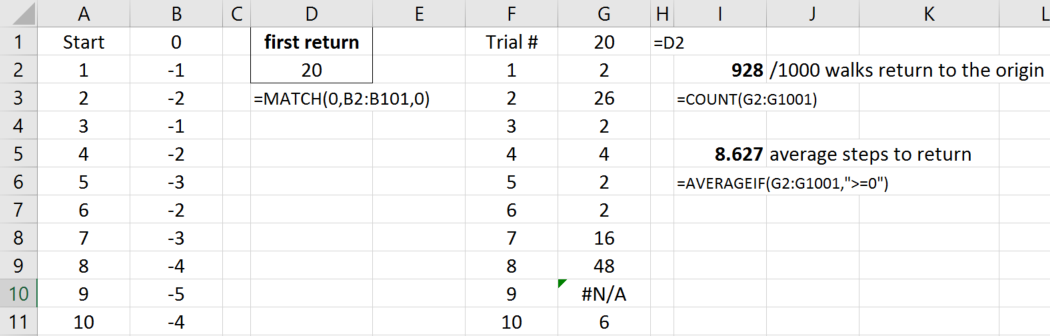
\includegraphics[width=\textwidth]{fig/3_randomwalk_3.png}
	\caption{1000 random walks of length 100. \label{fig:3_randomwalk_3}}
\end{figure}


\begin{figure}[htbp!]
	\centering
	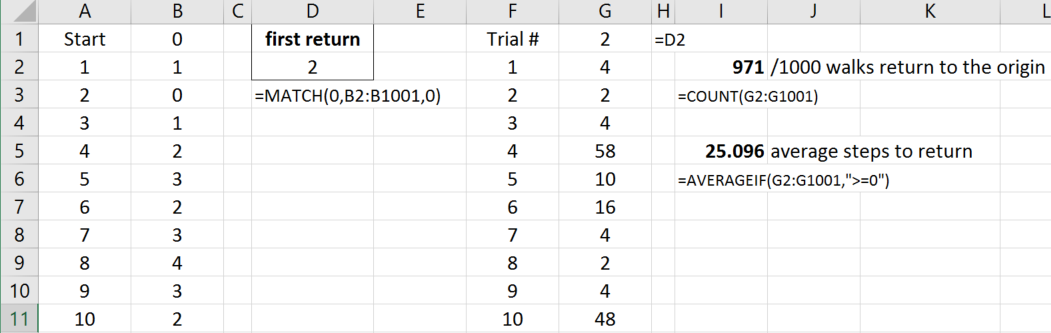
\includegraphics[width=\textwidth]{fig/3_randomwalk_4.png}
	\caption{1000 random walks of length 1000. \label{fig:3_randomwalk_4}}
\end{figure}

A \texttt{\#N/A} entry denotes that the walk did not return to 0, while the \texttt{COUNT} function counts the number of cells in the data table that have numbers.
Observe that only $92.2\%$ of the 100-step walks returned to 0, while $97.4\%$ of the 1000-step walks did.
This suggests that all the random walks will eventually return to zero, but some take a long time to do so.

We can also keep track of the average number of steps it takes for a walk to return to zero.
We calculate this using \texttt{AVERAGEIF(G2:G1001,``>=0'')}, which takes the average of the cells in the data table while ignoring the cells with \texttt{\#N/A}.
Increasing the length of the walk thus increases the number of walks that do return to zero, but the average number of steps continues to increase as we increase the number of steps and capture the walks that take a long time to return to zero.
In fact, it is possible to prove (with considerable effort) that while walks will eventually return to zero, the expected time to return is infinite.
This is because the average time is dominated by a few long walks, a fact that we can appreciate experimentally.

\newpage

Using Python we generated 100,000 walks for each of the following lengths, and obtained these results. (The code to implement this can be found after the exercises.)

\begin{center}
\begin{tabular}{rcr}
length of walks & \% returning & average time to return\\
\hline
10 & $73.513\%$ & $3.27$ \\
100 & $92.049\%$ & $8.57$ \\
1000 & $97.471\%$ & $25.86$ \\
10000 & $99.183\%$ & $76.30$ \\
100000 & $99.744\%$ & $238.20$ \\
1000000 & $99.932\%$ & $786.75$ \\
10000000 & $99.976\%$ & $2949.73$ \\
\end{tabular}
\end{center}

Observe that even for walks with ten million steps there is a small fraction that do not return to zero.

Using the same simulation we can also investigate the expected distance from the origin after a fixed number of steps.
Try this yourself for walks of 100 steps and then 1000 steps, and try to understand the pattern.



\subsection{Random Walks on a Grid}

Suppose now that we start at the origin $(0,0)$ in 2-dimensional space, and consider the lattice of integer points $\{(x,y) : x,y \text{ integers}\}$.
Assume that there is an equal probability (of $0.25$ each) of moving to an adjacent integer point at each step.
We would now like to estimate similar quantities as in the 1-dimensional case: what is the probability of returning to the origin?
What is the expected distance from the origin for a walk of fixed length?
We remark that the expected time to return to zero must be $\infty$ as it is that for each coordinate separately.
Moreover there are multiple notions of distance we can consider -- the Euclidean distance ($\sqrt{x^2 + y^2}$) and the Manhattan distance ($|x| + |y|$) are examples.

\begin{figure}[h]
	\centering
	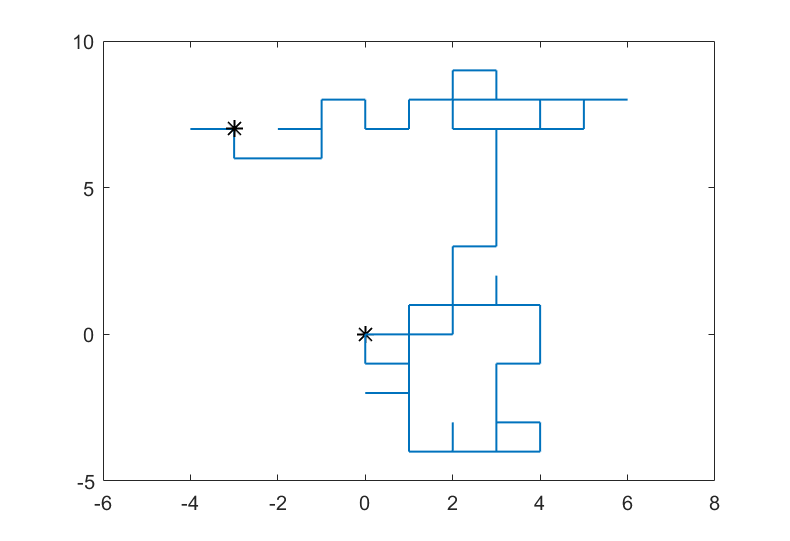
\includegraphics[width=0.5\textwidth]{fig/3_random2D_2.png}
	\caption{100 steps of a random walk on a grid, visualized. \label{fig:3_random2D_2}}
\end{figure}


To simulate this in Excel, we now need to keep track of two columns, one each for the $x$- and $y$-coordinate.
Refer to Figure~\ref{fig:3_random2D_1} for the formulas used (note that \texttt{F2} has a formula that changes based on the length of this walk, which is input in \texttt{F5}).

\vspace{0.5cm}

\begin{figure}[h]
	\centering
	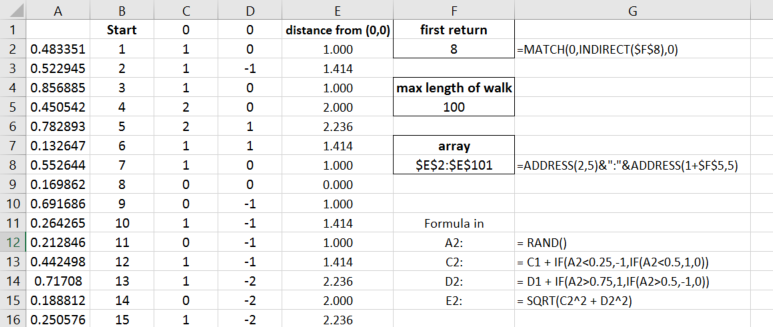
\includegraphics[width=\textwidth]{fig/3_random2D_1.png}
	\caption{100 steps of a random walk on a grid. \label{fig:3_random2D_1}}
\end{figure}

\vspace{0.5cm}

Using a data table, we simulate a thousand random walks of length 100 and 1000.
Observe that the percentages are much smaller than what we saw in the one-dimensional case: $58.1\%$ for walks of length 100, and $69.9\%$ for walks of length 1000.
Even increasing the length to 5000 only increases this observed frequency to $71.8\%$ (try it yourself and see what percentages you get!).

\vspace{0.5cm}

\begin{figure}[h]
	\centering
	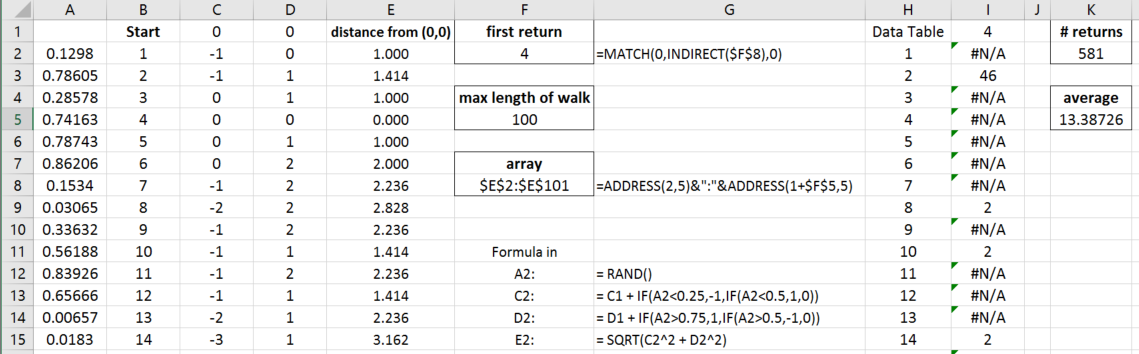
\includegraphics[width=\textwidth]{fig/3_random2D_3.png}
	\caption{1000 random walks of length 100. \label{fig:3_random2D_3}}
\end{figure}

\vspace{0.5cm}

\begin{figure}[h]
	\centering
	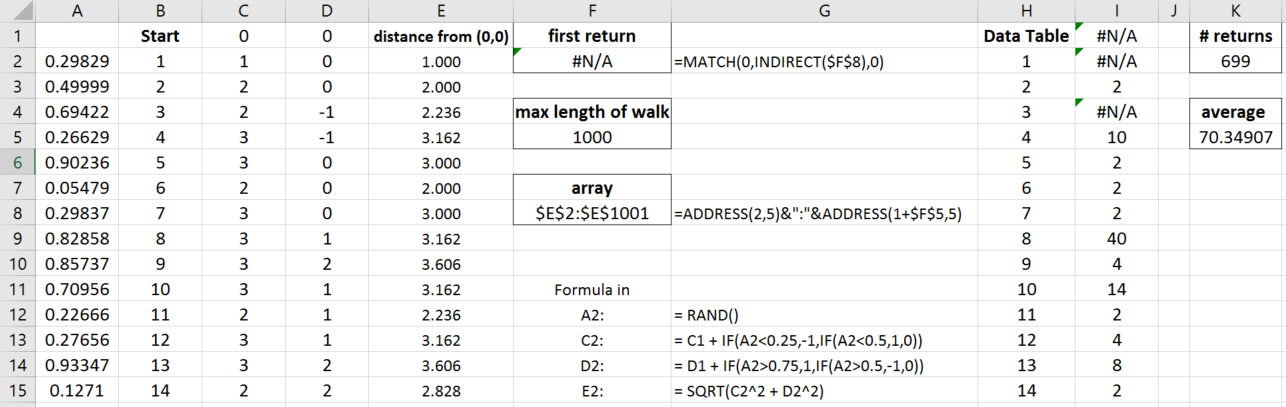
\includegraphics[width=\textwidth]{fig/3_random2D_4.png}
	\caption{1000 random walks of length 1000. \label{fig:3_random2D_4}}
\end{figure}

Based on this, it is hard to tell if the probability of returning to the origin might be smaller than 1 -- however, it has been shown analytically that as the length of the walk approaches infinity, this probability approaches 1.\footnote{See the article on \emph{P\'olya's Random Walk Constants} at \\ \url{http://mathworld.wolfram.com/PolyasRandomWalkConstants.html}.}
This illustrates one difficulty of performing simulations -- if the sample size is too small, the results might not necessarily reflect the true behaviour accurately.
In this example, even working with walks of length 5000, we still found a return rate of smaller than $75\%$.
On the other hand, it is hard to run a large number of experiments on Excel, as we don't have a good way to truncate walks that have already returned to zero.
Other programming languages are better for this purpose, however the trade-off between accuracy and running time remains.

\vspace{1cm}

\begin{center}
	\textbf{EXERCISES}
\end{center}

\begin{enumerate}[label={3.\arabic*},leftmargin=1cm]
	\item Consider the following experiment: roll three 6-sided dice at the same time, and let $X$ be the random variable that is equal to the number of different outcomes seen. For example, a roll of $\{3, 5, 5\}$ gives $X = 2$. Estimate the probability distribution for $X$ using an Excel simulation. Then, by enumerating all possibilities completely, determine the exact probabilities.
	\item Another puzzle from \emph{The Riddler}:
		\begin{quote}
			You and I stumble across a 100-sided die in our local game shop.
		We know we need to have this die -- there is no question about it -- but we're not quite sure what to do with it.
		So we devise a simple game: We keep rolling our new purchase until one roll shows a number smaller than the one before.
		Suppose I give you a dollar every time you roll.
		How much money do you expect to win?\footnote{\url{https://fivethirtyeight.com/features/how-long-will-it-take-to-blow-out-the-birthday-candles/}, January 13, 2017.}
	\end{quote}
		Estimate this quantity using a simulation.
	      \item The probability that two positive integers picked randomly are coprime (that is, they share no divisors other than 1) is $\frac{6}{\pi^2}$.
		Provide estimates for $\pi$ by taking 100, 1000, and 10000 pairs of integers from the ranges $\{1,2,\ldots,100\}$, $\{1,2,\ldots,1000\}$, and $\{1,2,\ldots,10000\}$.\footnote{This video by mathematician-comedian Matt Parker on his \emph{Youtube} channel \emph{standupmaths} demonstrates this process: \url{https://www.youtube.com/watch?v=RZBhSi\_PwHU} .}
	\item For a random walk in one dimension, estimate the expected distance from the origin after 200, 500, and 1000 steps by generating 1000 walks for each case.
	\item \textbf{Biased random walks}. Consider a one-dimensional random walk where you move one unit to the left with probability $p$ and one unit to the right with probability $1 - p$.
		Simulate this for $p = 0.6$.
		Do you expect all walks to return to the origin in this case?
		How about if $p = 0.8$?
	\item \textbf{Biased random walks}. Consider a one-dimensional random walk where at the origin, you move one unit to the left or right with equal probability, but everywhere else, you move \emph{towards the origin} with probability $p$, and \emph{away from the origin} with probability $1-p$.
		Simulate this for $p = 0.4$ and $p = 0.6$, and explain your results.
		Note that the formula to generate the next step is more involved, since you have to deal with three different cases.
	\item \textbf{Random walks in three dimensions}.
		Consider a random walk in 3D, where you start at the origin $(0,0,0)$, and with equal probability move $1$ or $-1$ units in one of the coordinate directions.
		Simulate this in Excel for a maximum length of 100 steps, and generate 100 walks using a data table. How many return to the origin?
		Try to generate longer walks (as far as your computer allows).
		Can you make any conclusions?

\end{enumerate}


{\small

\textbf{Python code for generating random walks}
\vspace{-0.5cm}

\begin{verbatim}
from __future__ import division
import random as rd

def randwalk(N,p=0.5,marker=0):
# Function for generating a random walk
# Input: N, p (prob of -1 step), marker (starting point)
#      *defaults are p = 0.5 and marker = 0
# Output: number of steps to first return to origin 
#         (or 0 if it does not return)
    current = marker # Initialize
    count = 0
    while count < N:
        # Generate random numbers, and move left or right
	# corresponding to probabilities
        r = rd.random()
        if r < p:
            current -= 1
        else:
            current += 1
        count += 1
        if current == 0:
            return count
    return 0


# Now aggregate up to M walks, and take return rate in % 
# and the average # steps to return

# Initialize parameters
N = 100
p = 0.5 
marker = 0
M = 100000 # Number of walks to aggregate

total_returns = 0
total_steps = 0
counter = 0

while counter < M:
    steps = randwalk(N,p,marker)
    if steps > 0:
        total_returns += 1
        total_steps += steps
    counter += 1

average_steps = total_steps/total_returns
return_rate = 100*total_returns/M

print "%d random walks of length %d were generated." % (M, N)
print "%7.4f%% of all walks returned to 0." % (return_rate)
print "On average it took %10.2f steps to return." % (average_steps)
\end{verbatim}

}

